\chapter{薛定谔方程与波函数}\label{ch:b2:schrodinger-wave-functions}

让电子逐个射向一对狭缝，并记录每个电子落在何处：
这里一个点，那里一个点，看似随机——而在一万个
点之后，便出现了杨氏实验的干涉条纹，仿佛每个电子
曾同时穿过两条狭缝，并与自身发生了干涉。本科一年级分册的
最后一章已经接触过这种奇异性：光
以光子的形式出现，物质具有波长 $\lambda = h/p$，位置与
动量不能同时确定。然而上一章没有给出
\emph{方程}——即描述与粒子相伴之波如何演化的规律，
正如牛顿定律描述轨迹如何演化。这一方程由
薛定谔（1926 年）提出。有了它，量子描述
才成为可计算的理论：人们写出\emph{\omterm{def:b2:schrodinger-wave-functions:psi}{波函数}}，
$\psi(x,t)$，其模的平方即找到粒子的概率，
然后求解一个线性偏微分方程。本章
给出该方程，解释 $\psi$ 的含义及其不含义，
求出\omterm{thm:b2:schrodinger-wave-functions:stationary}{定态}与自由粒子的波包，
并说明牛顿力学在何处重新出现——
对于比分子更重的一切物体。

\begin{omfigure}
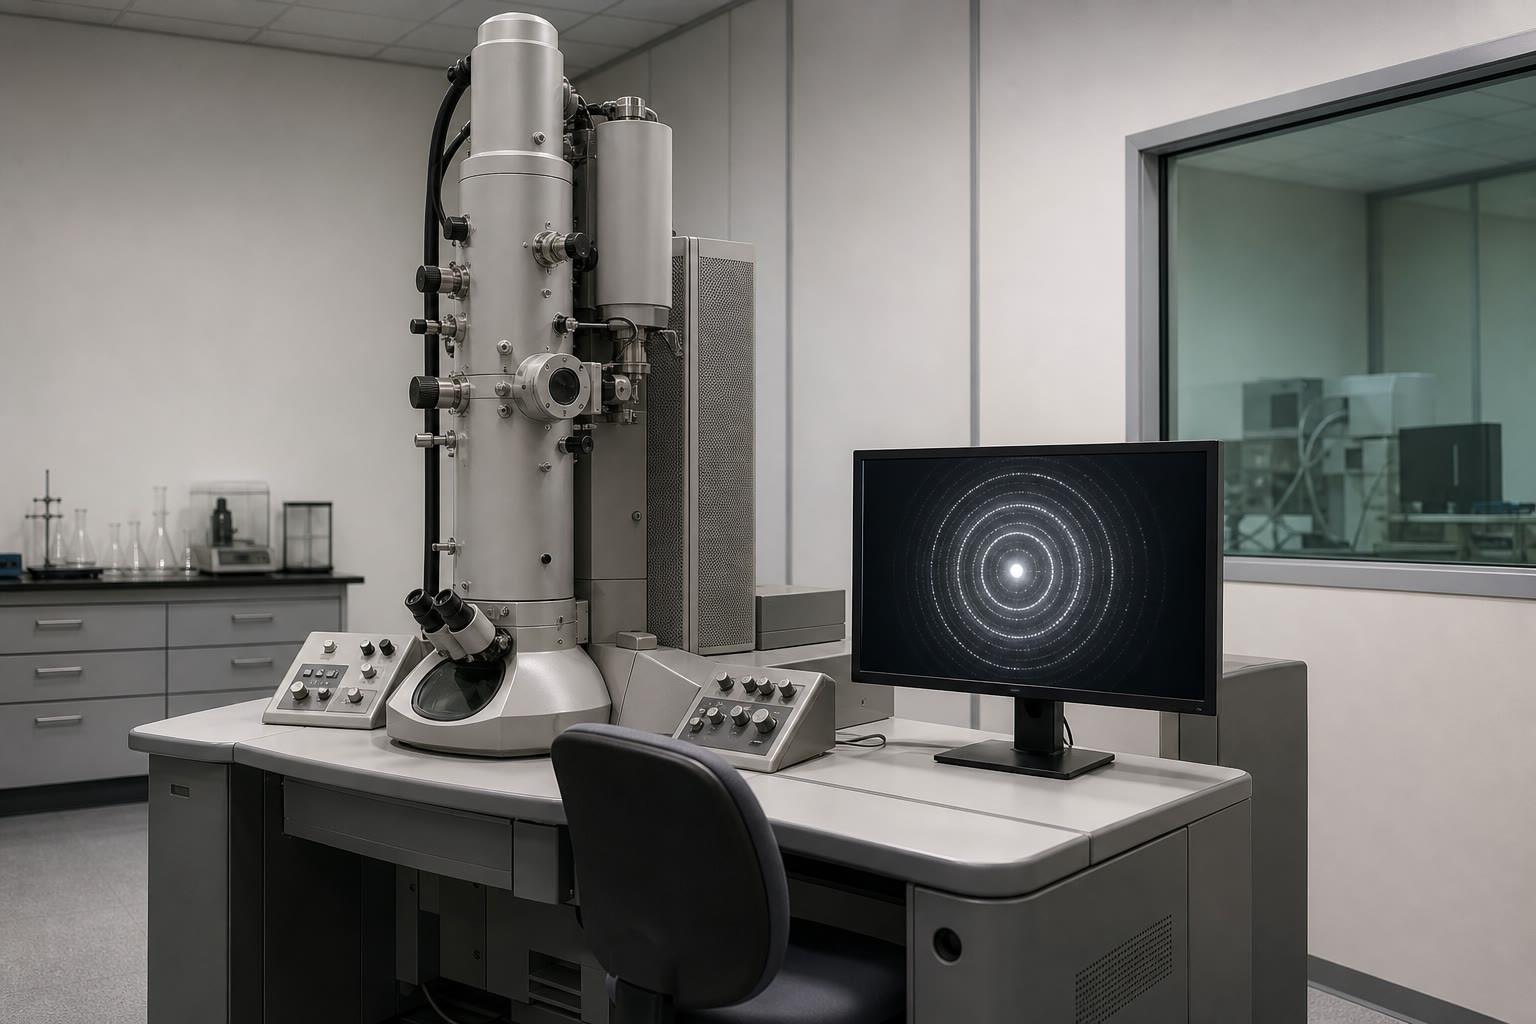
\includegraphics[width=0.58\linewidth]{images/book4/ai/b4-30-electron-microscope.jpg}

{\small 透射电子显微镜：电子被加速至
一百千伏，其波长仅为几皮米，它们的
\omterm{def:b2:schrodinger-wave-functions:psi}{波函数}经磁透镜聚焦，成像出
晶体中的原子。}
\end{omfigure}

\section{本科一年级分册留给我们的内容}

\begin{proposition}[粒子即波]\label{prop:b2:schrodinger-wave-functions:recap}
频率为 $\nu$ 的光子具有能量 $E = h\nu = \hbar\omega$，动量
$p = h/\lambda = \hbar k$；动量为 $p$ 的实物粒子表现为波长
$\lambda = h/p$ 的波（德布罗意），且同样有 $E =
\hbar\omega$ 与 $p = \hbar k$——电子在晶体上的\omterm{def:b2:diffraction:huygens}{衍射}、
中子乃至分子的干涉实验都证实了这一点；并且
任何态的位置与动量都不能同时任意精确，满足 $\Delta x\,\Delta p
\ge \hbar/2$（海森堡）。取 $\hbar = h/2\pi = \qty{1.05e-34}{J.s}$：
能量为 \qty{100}{eV} 的电子，其 $\lambda = \qty{0.12}{nm}$，
与一个原子的大小相当；质量为 \qty{1e-15}{kg}、速度为 \qty{1}{mm/s} 的尘埃颗粒，其 $\lambda =
\qty{7e-16}{m}$，小于原子核——它表现出经典行为。
\end{proposition}

\begin{proof}
由本科一年级分册回顾；现在的任务是
波的动力学。
\end{proof}

\begin{omfigure}
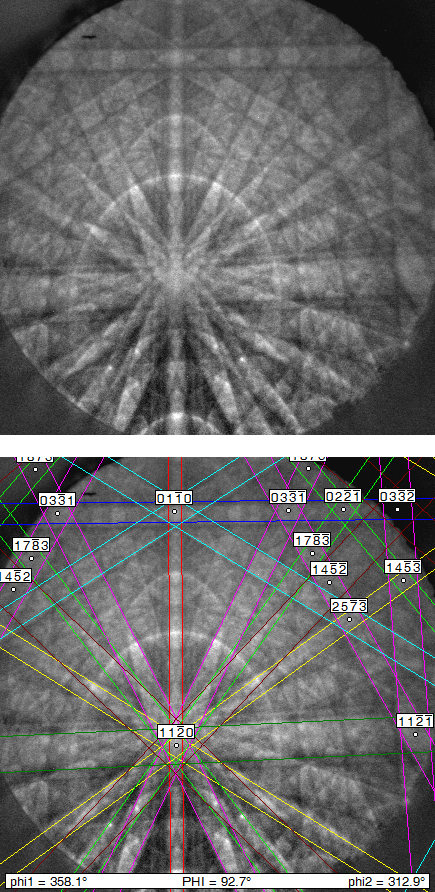
\includegraphics[width=0.4\linewidth, viewport=0 214 209 428, clip]{images/book4/electron-diffraction-nist.jpg}

{\small 电子显微镜中记录的电子\omterm{def:b2:diffraction:huygens}{衍射}图样（晶体的菊池图样）：波长为几皮米的电子被原子面\omterm{def:b2:diffraction:huygens}{衍射}——物质表现为波（NIST）。}
\end{omfigure}

\section{波函数}

\begin{definition}[波函数与玻恩定则]\label{def:b2:schrodinger-wave-functions:psi}
沿 $x$ 方向运动的粒子的状态，由复值的
\emph{波函数}\index{波函数} $\psi(x,t)$ 描述，使得
\[
\dd\mathcal P = |\psi(x,t)|^2\,\dd x
\]
是粒子在 $x$ 与 $x + \dd x$ 之间被找到的概率，
时刻为 $t$（\emph{玻恩定则}\index{玻恩定则}）；因此
有\emph{归一化} $\int_{-\infty}^{\infty}|\psi|^2\dd x = 1$，以及
期望值 $\langle x\rangle = \int x|\psi|^2\dd x$，$\Delta x^2 =
\langle x^2\rangle - \langle x\rangle^2$。波函数服从
\emph{叠加原理}\index{叠加原理}：若
$\psi_1$ 与 $\psi_2$ 是可能的态，则 $\alpha\psi_1 +
\beta\psi_2$（经归一化后）也是可能的态，且其概率中包含
干涉项 $2\operatorname{Re}(\alpha^*\beta\,\psi_1^*\psi_2)$。
整体相位因子 $\eu^{\iu\theta}$ 不产生任何影响；两个叠加分量之间的
相对相位则会改变干涉。
\end{definition}

\begin{remark}[$\psi$ 不是什么]\label{rem:b2:schrodinger-wave-functions:not}
$\psi$ 不是像 $\vect E$ 那样在空间中弥散的经典场，也不是
物质云：电子总是整体地出现在一个点上。
$\psi$ 是\emph{概率幅}，正是它发生干涉；
只有 $|\psi|^2$ 可被观测，且只能统计地观测，
即对相同制备的粒子重复实验。双缝上的点
均为单电子；条纹则由 $|\psi_1 +
\psi_2|^2$ 给出。
\end{remark}

\section{薛定谔方程}

\begin{theorem}[薛定谔方程]\label{thm:b2:schrodinger-wave-functions:equation}
质量为 $m$、处于势能 $V(x)$ 中的粒子，其
\omterm{def:b2:schrodinger-wave-functions:psi}{波函数}满足
\[
\iu\hbar\,\frac{\partial\psi}{\partial t} = -\frac{\hbar^2}{2m}\,\frac{\partial^2\psi}{\partial x^2} + V(x)\,\psi .
\]
该方程是线性的（满足\omterm{def:b2:schrodinger-wave-functions:psi}{叠加原理}），对时间为一阶（某一时刻的
\omterm{def:b2:schrodinger-wave-functions:psi}{波函数}决定了它此后所有时刻的值），并且是复的（$\psi$
不可能为实函数：其中的 $\iu$ 是本质的）。它是一条\emph{假设}，
其正当性由其推论来确立。
\end{theorem}

\begin{proof}
这是动机说明而非证明。动量确定的自由粒子，
即具有确定的 $p = \hbar k$ 与 $E = \hbar\omega$ 者，应为平面波 $\psi =
A\eu^{\iu(kx - \omega t)}$，对此有 $\iu\hbar\partial_t\psi = \hbar\omega\psi =
E\psi$，且 $-(\hbar^2/2m)\partial_x^2\psi = (\hbar^2k^2/2m)\psi = (p^2/2m)\psi$。
于是经典关系 $E = p^2/2m$ 由
方程 $\iu\hbar\partial_t\psi = -(\hbar^2/2m)\partial_x^2\psi$ 重现，并且自然的
推广 $E = p^2/2m + V$ 只需加上 $V\psi$。注意到
方程必须是线性的，方能对平面波的叠加成立，且
对时间为一阶并带有 $\iu$，使得时间依赖为 $\eu^{-\iu\omega t}$ 而非
$\cos\omega t$ 的形式——实的\omterm{thm:b2:waves-on-strings:equation}{波动方程}将
给出 $E^2 \propto p^4$。
\end{proof}

\begin{proposition}[概率守恒]\label{prop:b2:schrodinger-wave-functions:current}
概率密度 $\rho = |\psi|^2$ 与\emph{概率
流}\index{概率流}
\[
j = \frac{\hbar}{m}\operatorname{Im}\Big(\psi^*\frac{\partial\psi}{\partial x}\Big)
= \frac{\hbar}{2\iu m}\Big(\psi^*\partial_x\psi - \psi\,\partial_x\psi^*\Big)
\]
满足 $\partial_t\rho + \partial_xj = 0$：概率既不产生，
也不消失，且 $\int|\psi|^2\dd x$ 始终等于 $1$。对平面波
$A\eu^{\iu kx}$，$j = |A|^2\hbar k/m = \rho v$：即密度乘以速度，与
任何流动一样。
\end{proposition}

\begin{proof}
$\partial_t(\psi^*\psi) = \psi^*\partial_t\psi + \psi\,\partial_t\psi^*$；由
方程及其共轭，$\partial_t\psi = (\iu\hbar/2m)\partial_x^2\psi -
(\iu/\hbar)V\psi$，$\partial_t\psi^* = -(\iu\hbar/2m)\partial_x^2\psi^* +
(\iu/\hbar)V\psi^*$；$V$ 项相消，其余为 $(\iu\hbar/2m)(\psi^*
\partial_x^2\psi - \psi\,\partial_x^2\psi^*) = -\partial_xj$。
\end{proof}

\begin{proposition}[动量、期望值与经典极限]\label{prop:b2:schrodinger-wave-functions:ehrenfest}
态的动量由算符 $\hat p =
-\iu\hbar\,\partial_x$（对平面波给出 $\hbar k$）：$\langle
p\rangle = \int\psi^*(-\iu\hbar\partial_x\psi)\dd x$，能量则由 $\hat H
= -(\hbar^2/2m)\partial_x^2 + V$，期望值满足
（埃伦费斯特）
\[
\frac{\dd\langle x\rangle}{\dd t} = \frac{\langle p\rangle}{m}, \qquad
\frac{\dd\langle p\rangle}{\dd t} = -\Big\langle\frac{\dd V}{\dd x}\Big\rangle :
\]
波包中心在 $V$ 至多为二次式时严格遵循牛顿定律，
而只要波包的宽度相对于 $V$ 变化的尺度足够窄，便近似成立
——即经典极限，
对任何宏观物体都成立，因为 $\hbar$ 极小。
\end{proposition}

\begin{proof}
对 $\langle x\rangle = \int x|\psi|^2$ 求导，利用 $\partial_t\rho =
-\partial_xj$，分部积分得 $\dd\langle x\rangle/\dd t = \int j\,\dd x
= \langle p\rangle/m$。第二式是同样的计算，
只是高一阶（在本阶段不加证明地承认）。
\end{proof}

\section{定态}

\begin{theorem}[定态]\label{thm:b2:schrodinger-wave-functions:stationary}
若 $V$ 不依赖于时间，则方程具有
分离变量形式的解：
\[
\psi(x,t) = \varphi(x)\,\eu^{-\iu Et/\hbar}, \qquad
-\frac{\hbar^2}{2m}\,\varphi'' + V\varphi = E\varphi
\]
（\emph{定态薛定谔方程}\index{薛定谔方程!定态}
）：\emph{定态}\index{定态}
，具有确定能量 $E$，其概率密度
$|\varphi|^2$ 不随时间移动。能量 $E$ 若使 $\varphi$
可接受（有界，对束缚态须可归一化），
则为\emph{能级}；一般解为叠加 $\psi =
\sum_nc_n\varphi_n(x)\eu^{-\iu E_nt/\hbar}$，两能级的叠加
其密度以\emph{玻尔频率}\index{玻尔频率}
振荡，$\nu_{21} = (E_2 - E_1)/h$，即原子所发射
或吸收的光的频率。
\end{theorem}

\begin{proof}
代入 $\varphi(x)f(t)$：$\iu\hbar f'/f = (-\hbar^2\varphi''/2m + V\varphi)/\varphi$，
关于 $t$ 的函数等于关于 $x$ 的函数，故为常数 $E$；$f
= \eu^{-\iu Et/\hbar}$。对两个能级，$|c_1\varphi_1\eu^{-\iu E_1t/\hbar} +
c_2\varphi_2\eu^{-\iu E_2t/\hbar}|^2 = |c_1\varphi_1|^2 + |c_2\varphi_2|^2 +
2\operatorname{Re}(c_1^*c_2\varphi_1^*\varphi_2\eu^{-\iu(E_2 - E_1)t/\hbar})$。
\omterm{thm:b2:schrodinger-wave-functions:stationary}{定态}的完备性在本阶段不加证明地承认。
\end{proof}

\begin{omfigure}
\begin{tikzpicture}
  \begin{axis}[omaxis, width=7.4cm, height=4.4cm, xmin=0, xmax=1, ymin=-1.3, ymax=1.5,
    xlabel={$x/L$}, ylabel={$\psi$}, xtick={0.5,1}, ytick=\empty, clip=false,
    legend style={font=\scriptsize, at={(0.5,-0.28)}, anchor=north, draw=none, fill=none, legend columns=3}]
    \addplot[omDef, thick, domain=0:1, samples=80] {1.41*sin(deg(pi*x))*cos(40)};
    \addlegendentry{$\operatorname{Re}\psi$}
    \addplot[omExo, thick, dashed, domain=0:1, samples=80] {-1.41*sin(deg(pi*x))*sin(40)};
    \addlegendentry{$\operatorname{Im}\psi$}
    \addplot[omThm, thick, domain=0:1, samples=80] {2*sin(deg(pi*x))^2-1.3};
    \addlegendentry{$|\psi|^2$（平移后）}
  \end{axis}
  \begin{scope}[xshift=9.4cm, yshift=1.3cm, >=stealth]
    \draw[->] (-1.5,0) -- (1.5,0) node[right, font=\scriptsize] {实};
    \draw[->] (0,-1.5) -- (0,1.5) node[above, font=\scriptsize] {虚};
    \draw[gray] (0,0) circle (1.1);
    \draw[->, omDef, very thick] (0,0) -- (-40:1.1);
    \draw[->, omDef] (1.1,0) arc (0:-40:1.1);
    \node[font=\scriptsize, omDef] at (-50:1.55) {$-Et/\hbar$};
    \node[font=\scriptsize] at (0,-1.85) {$\eu^{-\iu Et/\hbar}$};
  \end{scope}
\end{tikzpicture}

{\small \omterm{thm:b2:schrodinger-wave-functions:stationary}{定态}：空间分布 $\varphi(x)$（此处为势阱的
基态）乘以一个以 $E/\hbar$ 为速率旋转的\omterm{thm:b2:gratings:nwaves}{相量}；
实部与虚部相互转化，而
$|\psi|^2$ 保持不动。}
\end{omfigure}

\begin{omfigure}
\begin{tikzpicture}
  \begin{axis}[omaxis, width=9cm, height=4.4cm, xmin=0, xmax=1, ymin=0, ymax=2.6,
    xlabel={$x/L$}, ylabel={$|\psi|^2$}, xtick={0.5,1}, ytick=\empty, clip=false,
    legend style={font=\scriptsize, at={(0.5,-0.28)}, anchor=north, draw=none, fill=none, legend columns=3}]
    \addplot[omDef, thick, domain=0:1, samples=100] {(sin(deg(pi*x)))^2 + (sin(deg(2*pi*x)))^2 + 2*sin(deg(pi*x))*sin(deg(2*pi*x))};
    \addlegendentry{$t = 0$}
    \addplot[omThm, thick, dashed, domain=0:1, samples=100] {(sin(deg(pi*x)))^2 + (sin(deg(2*pi*x)))^2};
    \addlegendentry{$t = T_{21}/4$}
    \addplot[omExo, thick, domain=0:1, samples=100] {(sin(deg(pi*x)))^2 + (sin(deg(2*pi*x)))^2 - 2*sin(deg(pi*x))*sin(deg(2*pi*x))};
    \addlegendentry{$t = T_{21}/2$}
  \end{axis}
\end{tikzpicture}

{\small 势阱中两个最低态的叠加：概率密度
在两侧之间来回晃动，频率为\omterm{thm:b2:schrodinger-wave-functions:stationary}{玻尔频率}
$(E_2 - E_1)/h$——振荡的电荷，因此（见\cref{ch:b2:dipole-radiation}）
恰好以谱线频率辐射的\omterm{thm:b2:dipole-radiation:field}{振荡偶极子}。}
\end{omfigure}

\section{自由粒子：平面波与波包}

\begin{proposition}[自由粒子]\label{prop:b2:schrodinger-wave-functions:free}
当 $V = 0$ 时，\omterm{thm:b2:schrodinger-wave-functions:stationary}{定态}为平面波 $\eu^{\iu(kx -
\omega t)}$，其中
\[
E = \hbar\omega = \frac{\hbar^2k^2}{2m}, \qquad
v_\varphi = \frac{\omega}{k} = \frac{\hbar k}{2m}, \qquad
v_{\text{g}} = \frac{\dd\omega}{\dd k} = \frac{\hbar k}{m} = \frac{p}{m} :
\]
物质波是\emph{色散的}；\omterm{def:b2:dispersion-wave-packets:relation}{相速度}没有物理意义，
\emph{\omterm{prop:b2:dispersion-wave-packets:group}{群速度}}才是粒子的速度。平面
波不可归一化——动量完全确定的粒子
弥散于整个空间——因此实际粒子是一个\emph{波
包}\index{波包}，即在一段
$\Delta k$ 范围内的平面波叠加，局域于 $\Delta x \sim 1/\Delta k$ 之内，以 $v_{\text{g}}$ 运动并
\emph{扩散}：初始宽度为 $\sigma_0$ 的高斯波包在
时刻 $t$ 的宽度为
\[
\sigma(t) = \sigma_0\sqrt{1 + \Big(\frac{\hbar t}{2m\sigma_0^2}\Big)^2}, \qquad
\tau = \frac{2m\sigma_0^2}{\hbar} ,
\]
且 $\Delta x\,\Delta p = \hbar/2$ 在 $t = 0$ 时成立（为允许的最小值），
之后则更大。
\end{proposition}

\begin{proof}
\omterm{def:b2:dispersion-wave-packets:relation}{色散关系}由方程导出；$v_{\text{g}}$ 见
\cref{ch:b2:dispersion-wave-packets}。扩散公式来自
波包的傅里叶合成。每个分量 $\eu^{\iu kx}$
获得相位 $\eu^{-\iu\hbar k^2t/2m}$，带复系数的高斯积分
给出宽度不断增大的高斯函数；傅里叶
积分是本科三年级数学分册的内容，此处在本阶段不加证明地承认其结果。
从物理上看：波包包含的动量分布范围为 $\Delta p
= \hbar/2\sigma_0$，因此速度的分布范围为 $\Delta v = \hbar/2m\sigma_0$，
经过时间 $t$ 后，较快的分量比较慢的分量多跑出 $\Delta v\,t$
——公式正是这一意思。
\end{proof}

\begin{omfigure}
\begin{tikzpicture}
  \begin{axis}[omaxis, width=6.2cm, height=4.4cm, xmin=0, xmax=3, ymin=0, ymax=2.6,
    xlabel={$k$}, ylabel={$\omega$}, xtick=\empty, ytick=\empty, clip=false]
    \addplot[omDef, thick, domain=0:2.3, samples=60] {x*x/2};
    \addplot[omExo, dashed, domain=0.4:2.6] {1.5*x-1.125};
    \addplot[omThm, dashed, domain=0:2.8] {0.75*x};
    \fill (axis cs:1.5,1.125) circle (1.5pt);
    \node[font=\scriptsize, omExo, anchor=west] at (axis cs:0.15,2.5) {$v_{\text{g}} = \hbar k/m$（切线）};
    \node[font=\scriptsize, omThm, anchor=west] at (axis cs:2.3,1.5) {$v_\varphi = \hbar k/2m$};
    \node[font=\scriptsize] at (axis cs:0.8,1.5) {$\omega = \hbar k^2/2m$};
  \end{axis}
  \begin{axis}[omaxis, width=7cm, height=4.4cm, xmin=-2.5, xmax=10, ymin=0, ymax=1.15, xshift=6.8cm,
    xlabel={$x/\sigma_0$}, ylabel={$|\psi|^2$}, xtick=\empty, ytick=\empty, clip=false]
    \addplot[omDef, thick, domain=-2.5:10, samples=120] {exp(-(x-1)^2/2)};
    \addplot[omThm, thick, domain=-2.5:10, samples=120] {(1/1.41)*exp(-(x-3.5)^2/4)};
    \addplot[omExo, thick, domain=-2.5:10, samples=120] {(1/2.24)*exp(-(x-6)^2/10)};
    \node[font=\scriptsize, omDef, anchor=west] at (axis cs:1.3,1.0) {$t = 0$};
    \node[font=\scriptsize, omThm, anchor=west] at (axis cs:3.8,0.75) {$\tau$};
    \node[font=\scriptsize, omExo, anchor=west] at (axis cs:6.3,0.5) {$2\tau$};
  \end{axis}
\end{tikzpicture}

{\small 左：自由粒子的色散曲线，图中标出\omterm{prop:b2:dispersion-wave-packets:group}{群速度}
（切线）与\omterm{def:b2:dispersion-wave-packets:relation}{相速度}（与原点的连线），仅画出其
一半。右：高斯波包以 $v_{\text{g}}$ 运动并扩散
——其宽度增为 $\sqrt2$ 倍（时刻 $\tau = 2m\sigma_0^2/\hbar$），其
峰值降低，面积不变。}
\end{omfigure}

\begin{example}[谁会扩散]\label{ex:b2:schrodinger-wave-functions:spreading}
一个局域在 $\sigma_0 = \qty{1}{nm}$ 之内的电子：$\tau = 2m\sigma_0^2/\hbar
= \qty{1.7e-14}{s}$——经过一纳秒后，其波包宽为 \qty{60}{\micro m}
宽：孤立的电子不会保持原位；束缚于原子中时，
因势场将其束缚而不会扩散（即\omterm{thm:b2:schrodinger-wave-functions:stationary}{定态}）。
一粒质量为 \qty{1e-15}{kg}、局域在 \qty{1}{\micro m} 之内的尘埃颗粒：$\tau =
\qty{2e7}{s}$，约八个月；子弹则长于宇宙的年龄。
量子扩散是真实的，但对任何肉眼可见的物体都无法察觉。
\end{example}

\begin{remark}[能量与时间]\label{rem:b2:schrodinger-wave-functions:energytime}
仅在 $\Delta t$ 时间内存在的态——寿命为
$\tau$ 的激发态原子、长度为 $c\tau$ 的\omterm{prop:b2:scalar-light-model:coherence}{波列}，是一系列能量的叠加，
其能量分布范围为 $\Delta E \sim \hbar/\Delta t$：即
\cref{ch:b2:scalar-light-model}中\omterm{prop:b2:scalar-light-model:coherence}{波列}时长与其\omterm{prop:b2:scalar-light-model:coherence}{谱宽}之间的傅里叶关系，
现将其用于 $E = \hbar\omega$。寿命为
\qty{10}{ns} 的原子能级，其宽度为 $\Delta E = \qty{7e-8}{eV}$，自然
线宽为 \qty{16}{MHz}；\cref{ch:b2:laser}中的多普勒宽度
（\qty{1.5}{GHz}）在气体中将其掩盖，但在静止的冷原子或离子中
则不然。
\end{remark}

\begin{method}[波函数的应用]\label{meth:b2:schrodinger-wave-functions:method}
(1) 归一化；概率为区域上的 $\int|\psi|^2$。(2)
若 $V$ 不含时：设 $\varphi(x)\eu^{-\iu Et/\hbar}$，求解
\omterm{thm:b2:schrodinger-wave-functions:stationary}{定态}方程，并施加边界条件——即得能级。
(3) 将\omterm{thm:b2:schrodinger-wave-functions:stationary}{定态}叠加以描述演化；两能级的拍频为
$(E_2 - E_1)/h$。(4) 自由运动：$v_{\text{g}} = p/m$，扩散时间
$2m\sigma_0^2/\hbar$。(5) \omterm{prop:b2:schrodinger-wave-functions:current}{概率流}：$j = (\hbar/m)\operatorname{Im}(\psi^*\psi')$；
对于 $A\eu^{\iu kx} + B\eu^{-\iu kx}$，$j = (|A|^2 - |B|^2)\hbar k/m$（无交叉项）。
(6) 经典极限：埃伦费斯特定理，以及 $\lambda$ 与
仪器尺度的对比。
\end{method}

\section{练习}

\begin{exercise}[$\star$]\label{exo:b2:schrodinger-wave-functions:1}
求德布罗意波长：电子能量分别为 \qty{100}{eV}、\qty{10}{keV}、
\qty{100}{keV}（用 $p = \sqrt{2mE}$ 求动量，再说明末一种情形为何需要
修正）；热中子（\qty{25}{meV}，$m = \qty{1.67e-27}{kg}$）；
以 \qty{200}{m/s} 运动的 C$_{60}$ 分子（$m = \qty{1.2e-24}{kg}$）；一个
网球。其中哪些会表现出干涉？
\end{exercise}

\begin{exercise}[$\star$]\label{exo:b2:schrodinger-wave-functions:2}
设 $\psi(x) = A\eu^{-x^2/2a^2}$，求 $A$（利用 $\int\eu^{-u^2}\dd u = \sqrt\pi$）；
求 $\langle x\rangle$、$\Delta x$；粒子出现在
$|x| < a$（$\operatorname{erf}(1) = 0.84$）和 $|x| < 2a$（$0.9995$）区域内的概率。
\end{exercise}

\begin{exercise}[$\star$]\label{exo:b2:schrodinger-wave-functions:3}
验证 $\varphi(x)\eu^{-\iu Et/\hbar}$ 在 $\varphi$
满足\omterm{thm:b2:schrodinger-wave-functions:stationary}{定态}方程时满足原方程。求 $E = \qty{1}{eV}$ 时\omterm{thm:b2:gratings:nwaves}{相量}的频率；
对于相隔 \qty{2}{eV} 的两能级叠加态，求 $|\psi|^2$ 振荡的频率与
波长——以及所发出光的
频率与波长。
\end{exercise}

\begin{exercise}[$\star$]\label{exo:b2:schrodinger-wave-functions:4}
求扩散时间 $\tau = 2m\sigma_0^2/\hbar$，以及经过 \qty{1}{ns} 和
\qty{1}{s} 后的宽度：电子分别取 $\sigma_0 = \qty{1}{nm}$ 与 $\sigma_0 = \qty{1}{mm}$；
质子取 $\sigma_0 = \qty{1}{nm}$；一粒质量为 \qty{1e-12}{kg} 的微粒，
取 $\sigma_0 = \qty{1}{\micro m}$。为什么物体会停留在放置的地方？
\end{exercise}

\begin{exercise}[$\star\star$]\label{exo:b2:schrodinger-wave-functions:5}
\emph{电流。}（a）推导\omterm{thm:b2:fluid-kinematics:continuity}{连续性方程}。（b）求以下情形的 $j$：
$A\eu^{\iu kx}$、$A\sin kx$、$A\eu^{\iu kx} + B\eu^{-\iu kx}$。（c）
为什么在最后一种情形中，交叉项为零就意味着
反射流与入射流简单相减？（d）证明：对于实\omterm{def:b2:schrodinger-wave-functions:psi}{波函数}
$j = 0$，即束缚\omterm{thm:b2:schrodinger-wave-functions:stationary}{定态}不携带电流。
\end{exercise}

\begin{exercise}[$\star\star$]\label{exo:b2:schrodinger-wave-functions:6}
\emph{高斯波包。}$\psi(x,0) = A\eu^{\iu k_0x}\eu^{-x^2/4\sigma^2}$。（a）
求 $A$、$\langle x\rangle$、$\Delta x$。（b）求 $\langle p\rangle$，用 $\hat p =
-\iu\hbar\partial_x$。（c）承认 $\Delta p = \hbar/2\sigma$，验证
$\Delta x\Delta p = \hbar/2$。（d）由\omterm{thm:b2:fluid-kinematics:continuity}{连续性方程}证明 $\dd\langle x\rangle/\dd t = \langle
p\rangle/m$。
\end{exercise}

\begin{exercise}[$\star\star$]\label{exo:b2:schrodinger-wave-functions:7}
\emph{管中的电子。}电子经 \qty{100}{V} 加速后穿过
\qty{30}{cm} 的管道。（a）求速率、波长与飞行时间。（b）求
\omterm{def:b2:dispersion-wave-packets:relation}{相速度}与\omterm{prop:b2:dispersion-wave-packets:group}{群速度}；电子的速度是哪一个？（c）初始宽为
\qty{10}{\micro m} 的波包：求扩散时间与到达时的宽度。（d）
途中经过 \qty{0.3}{mm} 孔径的\omterm{def:b2:diffraction:huygens}{衍射}：求角展宽与屏上的
光斑。射线图像是否成立？
\end{exercise}

\begin{exercise}[$\star\star$]\label{exo:b2:schrodinger-wave-functions:8}
\emph{相位。}（a）证明 $\psi$ 与 $\eu^{\iu\theta}\psi$ 给出相同的
预测。（b）对于 $\psi = (\psi_1 + \eu^{\iu\alpha}\psi_2)/\sqrt2$，写出
$|\psi|^2$，并证明 $\alpha$ 有影响。（c）在双缝实验中，
$\psi_1$ 与 $\psi_2$ 是什么，以及屏上某点处
两者的相对相位由什么决定？（d）为什么探测电子经过了哪一条缝
会破坏干涉条纹？（定性地回答）
\end{exercise}

\begin{exercise}[$\star\star$]\label{exo:b2:schrodinger-wave-functions:9}
\emph{埃伦费斯特定理。}（a）对于 $V = \tfrac12m\omega^2x^2$，证明 $\langle
x\rangle$ 精确满足 $\ddot{\langle x\rangle} = -\omega^2\langle x\rangle$。
（b）对于 $V = mgx$，$\langle x\rangle$ 像石头一样下落。（c）对于一般的
$V$，何时有 $\langle V'(x)\rangle \approx V'(\langle x\rangle)$？（d）置于碗中的
\qty{1}{g} 小珠：估算使其表现出“量子”性质所需的波包尺度，
并与原子进行比较。
\end{exercise}

\begin{exercise}[$\star\star\star$]\label{exo:b2:schrodinger-wave-functions:10}
\emph{晃动。}在壁不可穿透的盒子 $0 < x < L$ 中，\omterm{thm:b2:schrodinger-wave-functions:stationary}{定态}为
$\varphi_n = \sqrt{2/L}\sin(n\pi x/L)$，$E_n =
n^2h^2/8mL^2$（见\cref{ch:b2:potential-wells-tunneling}）。取 $\psi =
(\varphi_1\eu^{-\iu E_1t/\hbar} + \varphi_2\eu^{-\iu E_2t/\hbar})/\sqrt2$。（a）
求 $|\psi|^2$ 作为时间的函数。（b）证明 $\langle x\rangle = L/2 -
(16L/9\pi^2)\cos\omega_{21}t$（利用 $\int_0^L x\sin(\pi x/L)\sin(2\pi x/L)\dd x
= -8L^2/9\pi^2$）。（c）电子，$L = \qty{1}{nm}$：求 $E_2 - E_1$、
振荡的频率与波长。（d）振荡的电荷会
产生什么（见\cref{ch:b2:dipole-radiation}）？由此对
谱线作出结论。
\end{exercise}

\begin{exercise}[$\star\star\star$]\label{exo:b2:schrodinger-wave-functions:11}
\emph{扩散，推导。}波包 $\psi(x,0) \propto \eu^{-x^2/4\sigma_0^2}$ 是
叠加 $\int g(k)\eu^{\iu kx}\dd k$，其中 $g(k) \propto
\eu^{-\sigma_0^2k^2}$（承认：高斯函数的傅里叶变换是
高斯函数，其宽度为 $1/2\sigma_0$（关于 $k$）。（a）写出 $\psi(x,t)$，即给每个分量
赋予相位 $\eu^{-\iu\hbar k^2t/2m}$。（b）对指数配方，
并承认 $\int\eu^{-\alpha k^2 + \beta k}\dd k = \sqrt{\pi/\alpha}\,
\eu^{\beta^2/4\alpha}$，对于实部为正的复数 $\alpha$，证明
$|\psi|^2$ 是宽度为 $\sigma(t) = \sigma_0\sqrt{1 + (\hbar t/2m
\sigma_0^2)^2}$ 的高斯函数。（c）解释 $\tau$，借助 $\Delta v = \Delta p/m$。（d）为何
真空中光子的波包不会扩散？
\end{exercise}

\begin{exercise}[$\star\star\star$]\label{exo:b2:schrodinger-wave-functions:12}
\emph{能量–时间。}（a）衰减为 $\eu^{-t/2\tau}\eu^{-\iu E_0t/\hbar}$ 的态
（概率为 $\eu^{-t/\tau}$）是能量的叠加：承认
其能量分布为全宽 $\Gamma =
\hbar/\tau$ 的洛伦兹线型，求 $\Gamma$ 在 $\tau = \qty{10}{ns}$（原子）、\qty{1e-8}{s}、
\qty{1e-23}{s}（强子共振态，单位为 MeV）时的值。（b）
求 \qty{10}{ns} 能级的自然线宽（以频率表示），并与多普勒宽度
\qty{1.5}{GHz} 比较。（c）如何观测自然宽度（冷原子、
囚禁离子）？（d）与所发出的
\omterm{prop:b2:scalar-light-model:coherence}{波列}的\omterm{prop:b2:scalar-light-model:coherence}{相干长度}相联系。
\end{exercise}

\section{问题：管中的电子与波包的扩散}

\begin{problem}[{周末问题——电子何时是粒子，
何时是波}]\label{pb:b2:schrodinger-wave-functions:1}
数据：$h = \qty{6.63e-34}{J.s}$，$\hbar = \qty{1.05e-34}{J.s}$，$m_{\text{e}} =
\qty{9.11e-31}{kg}$，$e = \qty{1.60e-19}{C}$，$m_{\text{p}} = \qty{1.67e-27}{kg}$。

\textbf{第一部分——阴极射线管。}
电子从热阴极逸出时能量可忽略，经
$U = \qty{20}{kV}$ 的电压加速，穿过 \qty{0.3}{mm} 的小孔，
打在距其 \qty{40}{cm} 远的屏上。
\begin{enumerate}
  \item 速率与动量（非相对论）；德布罗意波长。
  \item 动能是 $4\%$ 的 $mc^2$：非相对论
        处理对本题是否可接受？
  \item 到屏幕的飞行时间。
  \item 小孔的\omterm{def:b2:diffraction:huygens}{衍射}：角展宽 $\sim\lambda/a$，以及
        它在屏上形成的光斑；与一个像素
        （\qty{0.3}{mm}）比较。
  \item 小孔处的海森堡关系：$\Delta p_y \gtrsim \hbar/2a$ 给出
        相同的展宽——请验证。
  \item 沿束流方向宽 \qty{0.3}{mm} 的波包：扩散时间
        $2m\sigma_0^2/\hbar$ 及其在屏上的宽度。
  \item 偏转极板施加横向力：由埃伦费斯特定理，
        $\langle y\rangle$ 如何运动？由此可知该管是一个
        经典器件。
  \item 电子波的\omterm{def:b2:dispersion-wave-packets:relation}{相速度}；为何它与电子的速率不同，
        并不是悖论？
\end{enumerate}

\textbf{第二部分——波包。}
\begin{enumerate}[resume]
  \item 对宽度为 $\sigma_0$ 的高斯波包，求 $\Delta p$ 及
        速度的展宽 $\Delta v$。
  \item 求电子在 $\sigma_0 = \qty{0.1}{nm}$、
        \qty{1}{nm}、\qty{1}{\micro m} 时的扩散时间；质子在 \qty{1}{nm} 时的
        扩散时间；病毒（\qty{1e-17}{kg}）在 \qty{10}{nm} 时的扩散时间。
  \item 氢原子中的电子被局限在 \qty{0.1}{nm} 范围内，
        却不发生扩散：为什么？
  \item 能量为 \qty{1}{eV} 的自由电子，$\sigma_0 = \qty{1}{nm}$：
        在其宽度加倍之前运动了多远？与
        波长比较。
  \item 在金属中，传导电子是遍及整个晶体的波，$\lambda \approx
        \qty{0.5}{nm}$；它们在什么意义上
        是“离域”的？
  \item 能量为 \qty{100}{keV} 的电子显微镜，其 $\lambda \approx
        \qty{4}{pm}$，分辨率却只有 \qty{0.1}{nm}：为何（其磁透镜
        接受的半角约为 \qty{10}{mrad}）？
  \item 给出判据，判断一个物体必须用\omterm{def:b2:schrodinger-wave-functions:psi}{波函数}处理还是用
        牛顿力学处理。
\end{enumerate}

\textbf{第三部分——\omterm{thm:b2:schrodinger-wave-functions:stationary}{定态}与跃迁。}
电子被限制在 $0 < x < L = \qty{1}{nm}$ 之间；$\varphi_n =
\sqrt{2/L}\sin(n\pi x/L)$，$E_n = n^2h^2/8mL^2$。
\begin{enumerate}[resume]
  \item 以电子伏特表示 $E_1$、$E_2$、$E_3$；\omterm{thm:b2:schrodinger-wave-functions:stationary}{玻尔频率}
        $\nu_{21}$、$\nu_{31}$ 及相应的波长。
  \item 验证 $|\varphi_n\eu^{-\iu E_nt/\hbar}|^2$ 与时间无关；
        基态时电子最可能出现在何处？
  \item 对 $\psi = (\varphi_1\eu^{-\iu E_1t/\hbar} + \varphi_2\eu^{-\iu E_2t/\hbar})/
        \sqrt2$，求 $|\psi|^2$ 在 $t = 0$ 及 $t = T_{21}/2$ 时的值，并作草图。
  \item 求 $\langle x\rangle(t)$（已知 $\int_0^Lx\varphi_1\varphi_2\dd x = -16L/9\pi^2$）
        “晃动”的振幅。
  \item \omterm{thm:b2:dipole-radiation:field}{振荡偶极子} $e\langle x\rangle$ 辐射，其频率为何，
        这对谱线有何说明，
        对\omterm{thm:b2:schrodinger-wave-functions:stationary}{定态}的稳定性又说明了什么？
  \item 态 $\psi$ 的能量是 $E_1$、$E_2$，还是
        别的值？测量会得到什么结果？
\end{enumerate}

\textbf{第四部分——诠释。}
\begin{enumerate}[resume]
  \item 在单电子双缝实验中，何者是随机的，
        何者不是？
  \item 写出 $A\eu^{\iu kx}$ 的\omterm{prop:b2:schrodinger-wave-functions:current}{概率流}，并将其与
        单位长度上有 $n$ 个电子、速率为 $v$ 的电子束相联系。
  \item 薛定谔方程为何必须是复的，并且对时间为一阶的，
        （两条理由）？
  \item 用五行概括：\omterm{def:b2:schrodinger-wave-functions:psi}{波函数}、方程、
        \omterm{thm:b2:schrodinger-wave-functions:stationary}{定态}、波包与经典极限。
\end{enumerate}
\end{problem}
